\chapter{User guide}
\label{sec:userguide}
\index{CRAVA!userguide}

In this chapter, we describe how to build a \crava model file. The model file mainly follows the XML-format, but we also use the character '\#' for commenting, meaning that the rest of the line after such a character is read as comment. XML/files are built with start- and endtags, encapsulating toher tags or values. All model files start with \texttt{<crava>}, and end with \texttt{<crava>}. An example of a model file is given in \autoref{sec:crava-model-file}.

\section{Basic inversion}
\label{sec:basicinv}
\index{inversion!basic}
A primary ability for \crava is to run simple first-pass inversions. In this section, we describe how to build a model file for a simple inversion. We focus on how to get the key information into the program, whereas more detailed controls are discussed later, in \autoref{sec:advinvusr}. The key information elements for a \crava inversion run is:
\begin{itemize}
\item \hyperref[sec:basicseis]{Seismic data}.
\item \hyperref[sec:basicwave]{Wavelet}.
\item \hyperref[sec:basicnoise]{Signal/noise ratio}.
\item \hyperref[sec:basicvol]{Inversion volume}.
\item \hyperref[sec:basicbg]{Background model}.
\item \hyperref[sec:basiccorr]{Correlation structures}.
\end{itemize}
Since \crava is designed to estimate any information that is not given, well data must also commonly be included.

\subsection{Survey information}
All information regarding the seismic data is gathered under the \kw{survey}\kwindex{survey} tag. This includes the file names for seismic data files, wavelet information and signal-to-noise ratio for each angle gather. As an example, it may look like this:
\svex{ex:survey}
<crava>
<survey>
  <segy-start-time>  2500.0 </segy-start-time>
  <angle-gather>
    <offset-angle>     16.0 </offset-angle>
    <seismic-data>
      <file-name> ../input/seismic/Cube16.segy </file-name>
    </seismic-data>
  </angle-gather>
  <angle-gather>
    <offset-angle>     28.0 </offset-angle>
    <seismic-data>
      <file-name> ../input/seismic/Cube28.segy </file-name>
    </seismic-data>
  </angle-gather>
</survey>
</crava>
\end{verbatim}
\end{example}

The seismic data can be given on SegY-format, with a common offset time
specified by the keyword \kw{segy-start-time}\kwindex{segy-start-time}
if the offset is different from 0. The first value is used to
represent the interval from start-time to start-time + time-step, so
with a start-time of 100ms, and 4ms sampling, the first value is used
in the grid cell covering the interval 100-104ms. If we use seismic
data of another format than SegY, the \kw{segy-start-time} command is
not used.  

For each available angle, the rest of the information is gathered under an \kw{angle-gather} tag, one for each offset. The actual angle is given by \kw{offset-angle}\kwindex{offset-angle}.

\subsubsection{Seismic data}
\label{sec:basicseis}
The name of the seismic data file is given with \kw{file-name}, as seen in \autoref{ex:survey}. Naturally, seismic data is always required when running an inversion.
By default, \crava recognizes three SegY formats; Seisworks, Charisma and IESX, but you are also allowed to define your own format using the \kw{segy-format}\kwindex{segy-format} command. A standard format is given by \kw{standard-format}. Possible arguments are 'seisworks', 'iesx', 'charisma' or 'SIP'. Modifications to the chosen standard format can be given by the following commands: \kw{location-x}, \kw{location-y}, \kw{location-il}, \kw{location-xl} and \kw{bypass-coordinate-scaling}. For more information on how to use this, see \kw{segy-format} in the reference manual chapter.

 
Other file formats recognized by \crava are storm, Sgri and crava.



\subsubsection{Wavelet}
\label{sec:basicwave}
To invert the seismic data, we need a wavelet for each angle. This wavelet can be read from file, using the \kw{wavelet}\kwindex{wavelet} and \rkw{file-name}{file-name2} commands like this:
\svex{ex:wavelet}
  <angle-gather>
    <offset-angle>     16.0 </offset-angle>
    <seismic-data>
      <file-name> ../input/seismic/Cube16.segy </file-name>
    </seismic-data>
    <wavelet>
      <file-name> ../input/wavelets/wavelet16.txt </file-name>
    </wavelet>
  </angle-gather>
\end{verbatim}
\end{example}

We can read wavelets on JASON and NORSAR format.

The Ricker wavelet is implemented in \crava, and can be used by the command \kw{ricker}\kwindex{ricker}. The peak frequency is given as argument.

If the \kw{wavelet} command is not given, or given without \kw{file-name}, the wavelet is estimated. See \autoref{sec:waveestimp} for how this is done. If the wavelet is given on file, but unscaled, the command \kw{scale}\kwindex{scale} should be used if the scale is known, otherwise, the scale can be estimated by using the \kw{estimate-scale}\kwindex{estimate-scale} command. If none of these are specified, the wavelet will be used as it is on file.

\subsubsection{Signal/noise ratio}
\label{sec:basicnoise}
This ratio is given with \kw{signal-to-noise-ratio}\kwindex{signal-to-noise-ratio}. If this command is not given, the ratio is estimated. Note that we define the signal to noise ratio as the data variance divided by the error variance, where the data variance is model variance plus error variance.

\subsection{Inversion volume}
\label{sec:basicvol}
The volume used for inversion is given horizontally by a rectangle, and vertically bounded by a top and base surface. It is defined by the command \kw{output-volume}\kwindex{output-volume} under \kw{project-settings}. Typically, it may look something like this:
\svex{ex:volume}
<crava>
<project-settings>
  <output-volume>
    <utm-coordinates>
      <reference-point-x>  403050.0   </reference-point-x>
      <reference-point-y> 7211900.0   </reference-point-y>
      <length-x>              500.0   </length-x>
      <length-y>              500.0   </length-y>
      <angle>                  23.627 </angle>
      <sample-density-x>       50.0   </sample-density-x>
      <sample-density-y>       50.0   </sample-density-y>
    </utm-coordinates>

    <interval-two-surfaces>
      <top-surface>
        <time-file>     ../input/horizons/FlatTop_3100ms.storm </time-file>
      </top-surface>
      <base-surface>
        <time-file>    ../input/horizons/FlatBase_3600ms.storm </time-file>
      </base-surface>
      <number-of-layers> 125 </number-of-layers>
    </interval-two-surfaces>
  </output-volume>
</project-settings>
</crava>
\end{verbatim}
\end{example}

\subsubsection{Lateral extent}
The lateral extent of the inversion volume is given under one of the
the commands \kw{area-from-surface}\kwindex{area-from-surface},
\kw{utm-coordinates}\kwindex{utm-coordinates}, or
\kw{inline-crossline-numbers}\kwindex{inline-crossline-numbers}. The
command \kw{utm-coordinates} describes a rectangle, which may be
rotated relative to the seismic data. It has the following parameters,
which must all be specified: 
\begin{itemize}
\item \kw{reference-point-x}\kwindex{reference-point-x} is the UTM x-coordinate of one corner of the area.
\item \kw{reference-point-y}\kwindex{reference-point-y} is the UTM y-coordinate of the same corner.
\item \kw{length-x}\kwindex{length-x} is the extent of the area along the local x-axis.
\item \kw{length-y}\kwindex{length-y} is the extent of the area along the local y-axis.
\item \kw{angle}\kwindex{angle} is the angle between the direction of the UTM x-axis and the local x-axis. Positive angles are counterclockwise.
\item \kw{sample-density-x}\kwindex{sample-density-x} is the length of one grid cell along the local x-axis.
\item \kw{sample-density-y}\kwindex{sample-density-y} is the length of one grid cell along the local y-axis.
\end{itemize}
Note that if the grid has the same rotation as the input SegY cubes with seismic data, output SegY cubes will have correct inlines and crosslines. Otherwise, these numbers are just counting from the initial corner.
The command \kw{area-from-surface} contains only one parameter, \kw{file-name}\kwindex{file-name}, the name of a storm surface file defining the lateral extent of the inversion volume.
The last way to define the inversion area is by the command \kw{inline-crossline-numbers}\kwindex{inline-crossline-numbers}. By this command, the following parameters can be used:
\begin{itemize}
\item \kw{il-start}\kwindex{il-start} is the starting inline number.
\item \kw{il-end}\kwindex{il-end} is the ending inline number.
\item \kw{xl-start}\kwindex{xl-start} is the starting crossline number.
\item \kw{xl-end}\kwindex{xl-end} is the ending crossline number.
\item \kw{il-step}\kwindex{il-step} is the inline interval.
\item \kw{xl-step}\kwindex{xl-step} is the crossline interval.
\end{itemize}
The parameters \kw{il-start} and \kw{xl-start} must be set if this command is used, the other parameters are optional. If they are not given, the numbers are taken from the Segy file containing the first seismic cube.

The area commands may be skipped altogether. The area will then be taken from the first input seismic data file, and defined as the smallest rectangle that covers all present traces.

\subsubsection{Top and base surfaces}
The vertical extent is normally given by a top and a base surface in
time, under the command \kw{interval-two-surfaces}
\kwindex{interval-two-surfaces}, as shown in \autoref{ex:volume}. The
file name for the top surface is given under command
\kw{top-surface}\kwindex{top-surface}, \kw{time-file}, and the base
surface is given similarly under \kw{base-surface}
\kwindex{base-surface}, \kw{time-file}. The file format is binary
storm or ASCII irap. Top and base time values for the inversion
interval can be given as constants instead of files, by using the
command \kw{time-value}\kwindex{time-value}.   

These surfaces also define the default lateral correlation direction
for the elastic parameters, with the correlation being parallel to the
top surface at the top, and base surface at the base. Between this, we
create a top- and base-conform grid, so that the number of grid cells
in each trace is constant, although the interval thickness may
vary. This is shown in part B of
\autoref{fig:inversion-interval-types}. The inversion may be unstable
if the resolution varies too much in different traces, so we recommend
that no trace interval is larger than twice the shortest interval. The
number of layers between top and base is given by the command
\kw{number-of-layers} \kwindex{number-of-layers}.

%\begin{figure}
%  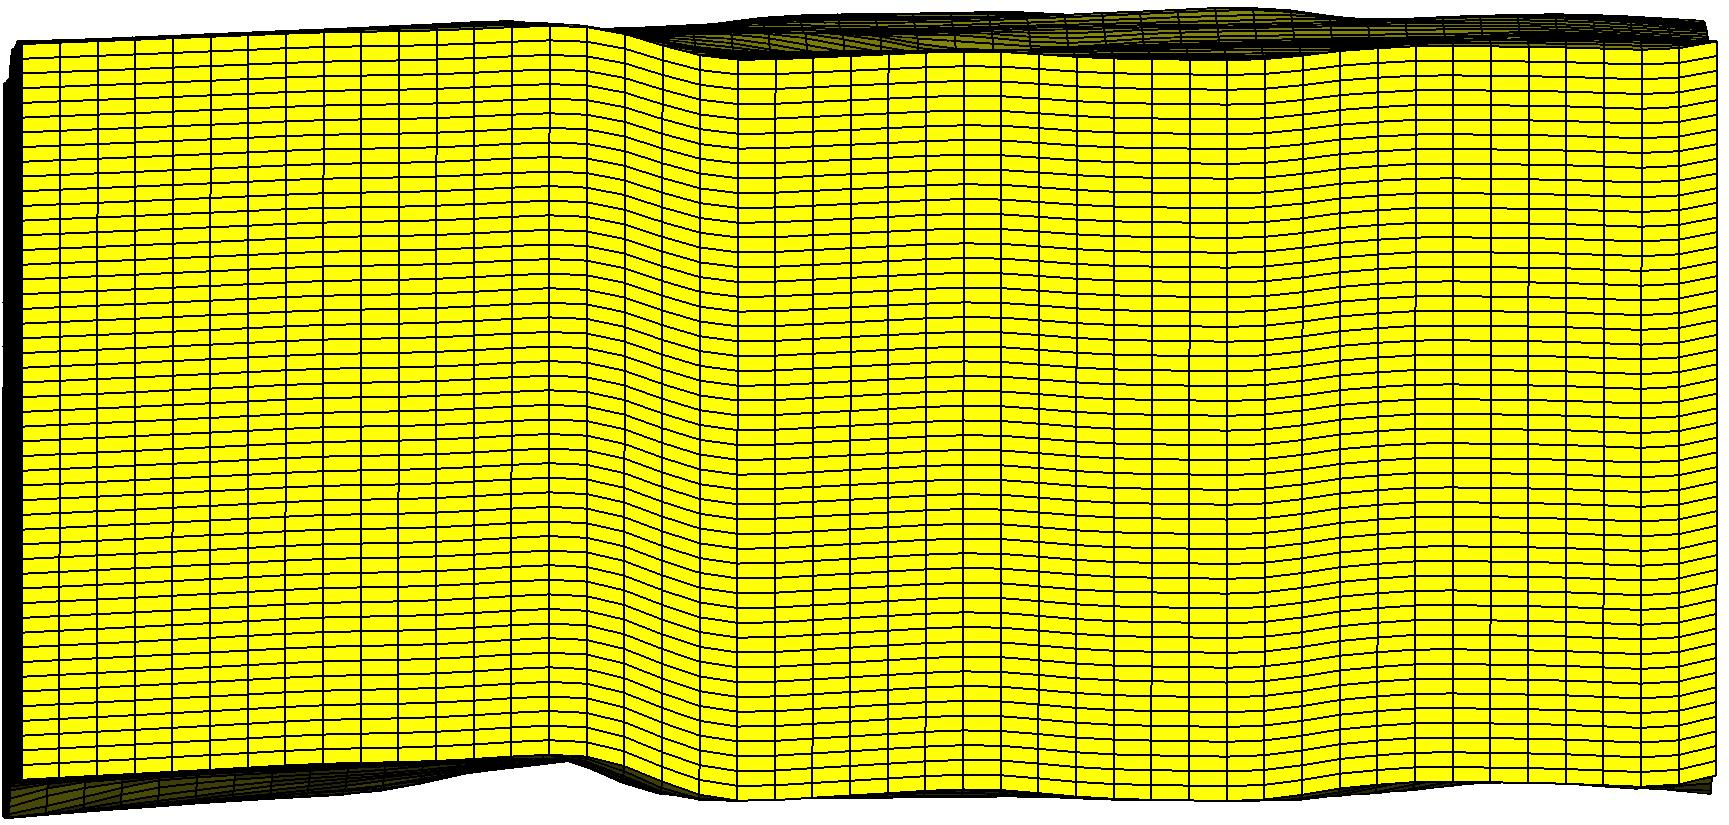
\includegraphics[width=.99\linewidth]{images/conformgrid}
%  \caption{The layer structure of a top- and base-conform grid.}
%  \label{fig:conformgrid}
%\end{figure}

\begin{figure}
  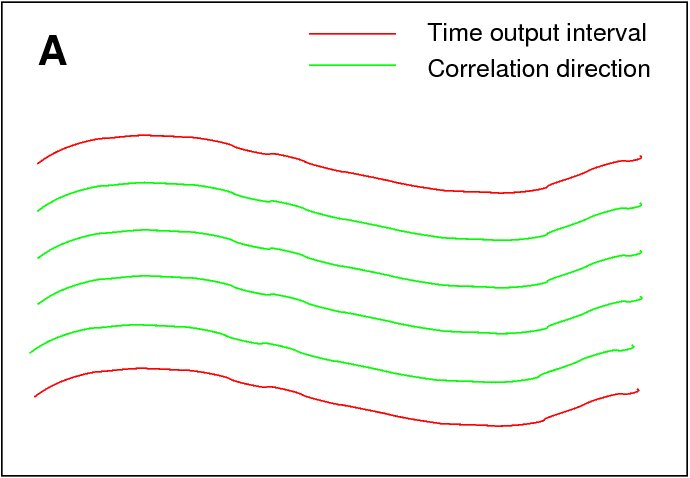
\includegraphics[width=.49\linewidth]{images/A_correlation_parallel}
  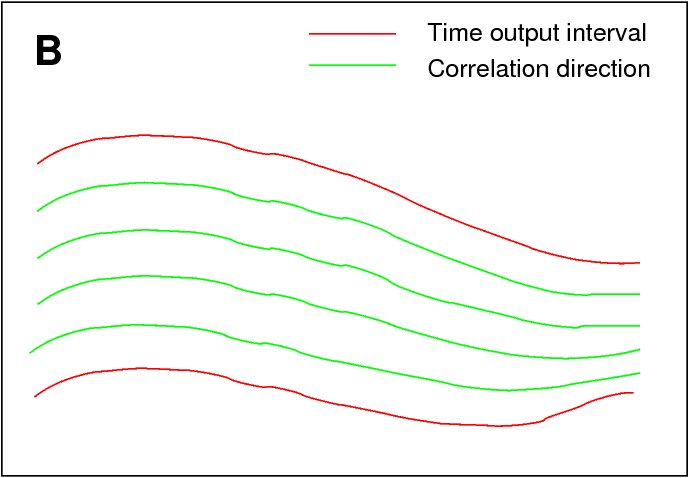
\includegraphics[width=.49\linewidth]{images/B_correlation_proportional}\\
  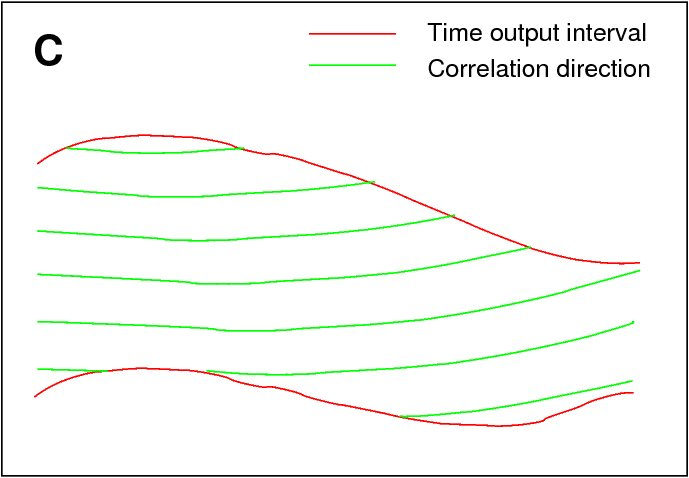
\includegraphics[width=.49\linewidth]{images/C_correlation_parallel_timecut}
  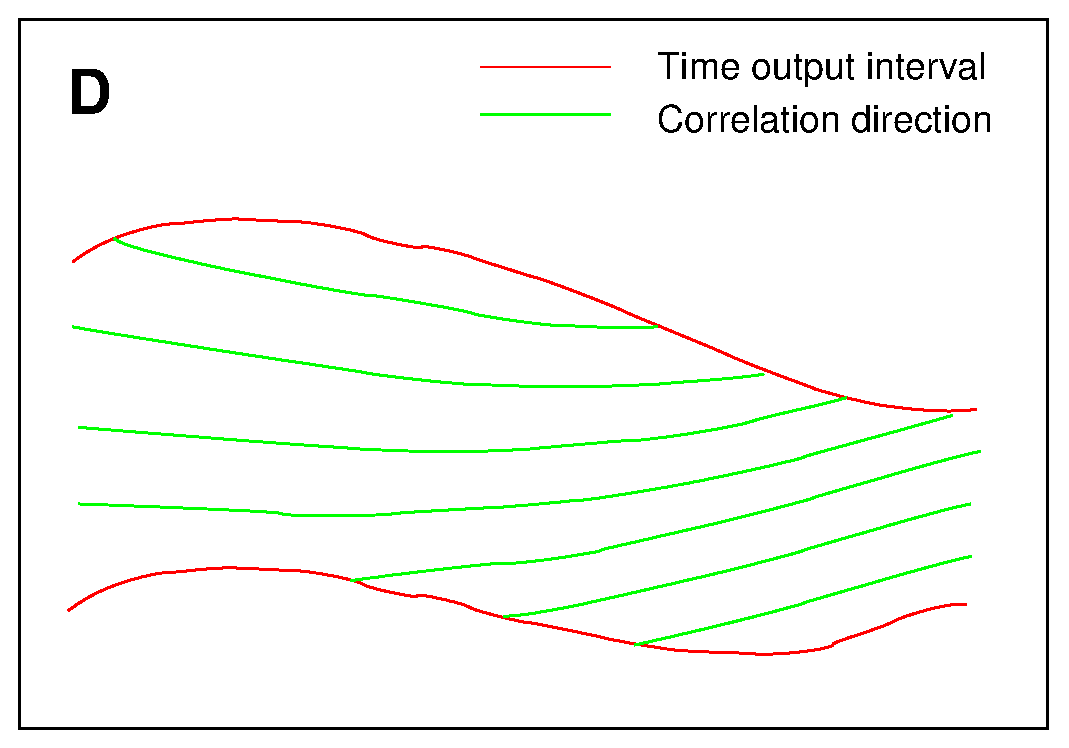
\includegraphics[width=.49\linewidth]{images/D_correlation_proportional_timecut}
  \caption{The layer structure of a (A) parallel top and base,
           (B) top- and base-conform compaction grid (C) Uniform correlation
           structure in a cut grid (D) Compactional correlation structure in a
           cut grid.} 
  \label{fig:inversion-interval-types}
\end{figure}

By specifying a correlation surface, the correlation direction can be
independent of the interval surfaces, see part C of
\autoref{fig:inversion-interval-types} and \autoref{sec:basiccorr}. If
this is done, there are no restrictions on the differences in interval
thickness.

The more flexible approach where a compactional correlation structure
is specified independent of the interval of interest (see part D of
\autoref{fig:inversion-interval-types})  is currently not implemented. 

If only one surface is known, the command \kw{interval-one-surface}
can be used to invert an interval with top and base parallel to this
surface. See \autoref{interval-one-surface} in the reference guide for
more details. Note that depth conversion and correlation surfaces will
not be available in this mode, so the lateral correlation will be
parallel to this surface as illustrated in part A of
\autoref{fig:inversion-interval-types}. 

\subsubsection{Depth conversion}\label{sec:depthconvusr}
The \kw{output-volume} command is also where the depth conversion is specified, since this also constitutes a volume although in depth. Since the lateral area obviously is the same, the additional information for depth conversion is given under \kw{interval-two-surfaces}. To do the depth conversion, one of the following must be given:
\begin{itemize}
\item Reference surface in depth (either top or base), and a velocity cube.
\item Both top and base surface in depth. In this case, we assume constant velocity along each trace, computed from the time and depth surfaces.
\item Both top and base surface in depth, and a velocity cube. In this case, we use the cube for relative velocity in a trace, and scale it to match the interval length.
\end{itemize}

Reference surfaces in depth are given with \kw{depth-file}\kwindex{depth-file} under \kw{top-surface} and/or \kw{base-surface}. The velocity cube can be read from a storm-file with the command \kw{velocity-field}\kwindex{velocity-field}. Alternatively, the command \kw{velocity-field-from-inversion}\kwindex{velocity-field-from-inversion} can be used to specify that Vp from inversion should be used for velocity. With depth conversion, the \kw{interval-two-surfaces} command may look like this:
\svex{ex:depthconv}
    <interval-two-surfaces>
      <top-surface>
        <time-file>     ../input/horizons/FlatTop_3100ms.storm </time-file>
        <depth-file>    ../input/horizons/FlatTop_3100ms.storm </depth-file>
      </top-surface>
      <base-surface>
        <time-file>    ../input/horizons/FlatBase_3600ms.storm </time-file>
        <depth-file>   ../input/horizons/FlatBase_3800ms.storm </depth-file>
      </base-surface>
      <velocity-field>        ../input/velocity/velocity.storm </velocity-field>
      <number-of-layers>                                   125 </number-of-layers>
    </interval-two-surfaces>
\end{verbatim}
\end{example}

\subsection{Prior model}
Since seismic data only contain information about relative elastic parameters, the absolute level needs to be set with a background model. In a Bayesian inversion setting, the background model is the prior expectation. We also need the prior covariance, which is given by the covariance of the parameters, the lateral correlation and the temporal correlation, as described in \autoref{sec:statmodthe}. In the model file, all this is gathered under the \kw{prior-model}\kwindex{prior-model} command, which may look something like this:
\svex{ex:priormodel}
<crava>
<prior-model>
  <background>
    <vp-file>
      ../../input/background/CravaBgVp.storm
    </vp-file>
    <vs-file>
      ../../input/background/CravaBgVs.storm
    </vs-file>
    <density-file>
      ../../input/background/CravaBgRho.storm
    </density-file>
  </background>
  <lateral-correlation>
    <variogram-type> genexp </variogram-type>
    <power>       1 </power>
    <angle>       0 </angle>
    <range>    2500 </range>
    <subrange> 2500 </subrange>
  </lateral-correlation>
</prior-model>
</crava>
\end{verbatim}
\end{example}

\subsubsection{Background model}
\label{sec:basicbg}
The background model is given under the \kw{background}\kwindex{background} command. It can be given from file, using \kw{vp-file}\kwindex{vp-file}, \kw{vs-file}\kwindex{vs-file} and \kw{density-file}\kwindex{density-file}. These files should either be on Storm, crava, Sgri or SegY format. Alternatively, constant values can be used for background model, specified with \kw{vp-constant}\kwindex{vp-constant}, \kw{vs-constant}\kwindex{vs-constant} and \kw{density-constant}\kwindex{density-constant}. Any combinations of files and constants are also ok. If none of these are given, the background model will be estimated.
\subsubsection{Covariances}
\label{sec:basiccorr}
As shown in \autoref{sec:statmodthe} the prior covariance structure for the elastic parameters consists of three parts:
\begin{enumerate}
\item A 3x3 covariance matrix for pointwise covariance between the parameters. May be read from ascii file using the command \kw{parameter-correlation}\kwindex{parameter-correlation}.
\item A temporal correlation vector, length equal to number of layers in grid, $n_t$. May be read from ascii file using the command \kw{temporal-correlation}\kwindex{temporal-correlation}.
\item A lateral correlation structure. May be given as a variogram using the command \kw{lateral-correlation}.
\end{enumerate}
By default, the two first are estimated from well data, and the lateral correlation structure is set to a isotrope exponential variogram with range 1000. The reason for the latter choice is that this is hard to estimate, see \autoref{sec:correstimp} for details. The most common to override is the lateral correlation, where the variogram used for petrophysical modelling is a good choice.
\subsection{Well data}
Unless all information about wavelet, signal to noise and correlations are specified, well data are needed for estimation. Wells are given with the command \kw{well-data}\kwindex{well-data}, and may look like this:
\svex{ex:welldata}
<crava>
<well-data>
  <log-names>
    <time>    TWT  </time>
    <dt>      DT   </dt>
    <dts>     DTS  </dts>
    <density> RHOB </density>
  </log-names>
  <well>
    <file-name> ../input/logs/ed6406_3-3_cut.rms    </file-name>
  </well>
  <well>
    <file-name> ../input/logs/ed6506_12-3_cut.rms   </file-name>
  </well>
  <well>
    <file-name> ../input/logs/ed6506_12-8_cut.rms   </file-name>
  </well>
  <well>
    <file-name> ../input/logs/ed6506_12-S4H_cut.rms </file-name>
  </well>
</well-data>
</crava>
\end{verbatim}
\end{example}
There are two main elements here. The first is a well log
interpretation, given by \kw{log-names}, which tells \crava which
headers to look for. The following logs are needed: 
\begin{itemize}
\item Two way time log, specified with \kw{time}\kwindex{time}.
\item Vp log, either given by \kw{vp}\kwindex{vp} or \kw{dt}\kwindex{dt}. The latter is used for DT-logs.
\item Vs log, either given by \kw{vs}\kwindex{vs} or \kw{dts}\kwindex{dts}. The latter is used for DTS-logs.
\item Density log, given by \kw{density}\kwindex{density}.
\end{itemize}
In addition, if facies probabilities are computed, a facies log is
needed. This is specified with \kw{facies}\kwindex{facies}. 

The wells are given with the command \kw{file-name} under
\kw{well}\kwindex{well}, which is given once for each well. The reason
for this is that additional information may be given for each
well. Well files should be on NORSAR or RMS-format. 

Each well may be moved to its optimal location using \kw{optimize-position}\kwindex{optimize-location-to} under \kw{well}\kwindex{well}, taking the arguments \rkw{angle}{angle3}\kwindex{angle} and \kw{weight}\kwindex{weight} allowing the user to assign different weights to the different angle gathers for each well. The maximum allowed offset and vertical shift for moving wells is specified in \kw{maximum-offset}\kwindex{maximum-offset} and \kw{maximum-shift}\kwindex{maximum-shift} under \kw{well-data}, with default values of 250 m and 11 ms, respectively.

The command \kw{synthetic-vs-log} tells whether the Vs log is synthetic. If not specified, it will be detected from correlation with Vp. The command \kw{filter-elastic-logs}\kwindex{filter-elastic-logs} is used to do multi-parameter-filtering of the elastic logs in this well after the inversion.

\subsection{I/O settings}
Two commands are used to specify the directory for input files. \kw{top-directory}\kwindex{top-directory} gives the working directory for the model file. 
The command \kw{input-directory}\kwindex{input-directory} is used to specify directory name for root directory for input files. The name is given relative to \kw{top-directory}.

Under \kw{advanced-settings}, the command \kw{use-intermediate-disk-storage} can be used to save memory use when running large \crava jobs. A built-in smart-swap is then activated. The option has largest effect on Windows. 

Under \kw{project-settings}, \kw{io-settings} and \kw{other-output}, the command \kw{error-file}\kwindex{error-file} writes all errors to a separate file, in addition to the log file. The command \kw{task-file}\kwindex{task-file} writes all tasks to a separate file, in addition to the log file. 
\subsection{Output}
Output is controlled under \kw{io-settings}\kwindex{io-settings} under
\kw{project-settings}. Here, you may set the output directory using
\kw{output-directory}\kwindex{output-directory}, and a prefix for all
output files using
\kw{file-output-prefix}\kwindex{file-output-prefix}. This prefix will
be added to all output files. 

Except for the log file which is placed directly under the
output directory, all files output by crava are placed in
sub-directories. These sub-directories are 

\svex{ex:output-directories}
output-directory / wells 
                 / background 
                 / wavelets 
                 / seismic 
                 / velocity 
                 / correlations 
                 / inversionresults 
\end{verbatim}
\end{example}

There are two main output formats: Grid output, controlled by
\kw{grid-output}\kwindex{grid-output}, and well output controlled by
\kw{well-output}\kwindex{well-output}. The output section may look
something like this: 
\svex{ex:iosettings}
<crava>
<project-settings>
  <io-settings>
    <file-output-prefix> CRAVA_ </file-output-prefix>
      <grid-output>
        <format>
          <segy> yes </segy>
        </format>
        <domain>
          <time>  yes </time>
          <depth> yes </depth>
        </domain>
        <elastic-parameters>
          <vp> yes </vp>
          <vs> yes </vs>
          <density> yes </density>
          <background> yes </background>
        </elastic-parameters>
      </grid-output>
      <well-output>
        <wells> yes </wells>
        <blocked-wells> yes </blocked-wells>
      </well-output>
  </io-settings>
</project-settings>
</crava>
\end{verbatim}
\end{example}

\subsubsection{Grid output}\kwindex{grid-output}
Different elastic parameters can be given as grid output. In addition, estimated background model may be written as grids. This is controlled by the \kw{elastic-parameters}\kwindex{elastic-parameters} command under \kw{grid-output}. See \autoref{elastic-parameters} for a full list of possible grids. If this command is not used, Vp, Vs and density will be written. Output of original and synthetic seismic data can be given by the \kw{seismic-data}\kwindex{seismic-data} command. Other output grids are given by the command \kw{other-parameters}\kwindex{other-parameters}, for example correlations.

The grid format may be controlled using \kw{format}\kwindex{format}. Here the yes/no parameters \kw{storm}, \kw{segy}, \kw{sgri}, \kw{crava} and \kw{ascii} can be used to decide if grids should be written on storm- (RMS), segy-, Sgri-, crava- or ascii-format. You may choose several formats for one run; all grids will be written on all selected formats. The Segy format can be controlled by the \kw{segy-format} command, in the same way as for input data, described in \autoref{sec:basicseis}. Note that correlation grids make sense only in storm format. Default output format is storm. The crava format is a binary format only to be used with \crava. It can be read and written from \crava, and is useful if the output from a \crava run should be used as input to another \crava run because the format is fast to read.

By using the \kw{domain}\kwindex{domain} option, output may be written in time domain (\kw{time}) or depth domain (\kw{depth}, requires parameters set under \kw{output-volume}, see \autoref{sec:depthconvusr}), or both. Again, correlation grids only make sense in time domain, which is default.

\subsubsection{Well output}\kwindex{well-output}
Some versions of filtered elastic parameters (Vp, Vs and density) in wells can be generated by the \kw{well-output} command. The wells can be given in two different formats, RMS or NORSAR. This is controlled by the \kw{format}\kwindex{format} command. The logs written are
\begin{itemize}
\item Raw elastic logs.
\item Elastic logs filtered to background frequency.
\item Elastic logs filtered to seismic frequency.
\item Elastic logs filtered with facies prediction filter (if available).
\item Facies log (if available).
\end{itemize}
The wells can either be written with original sampling density, using \kw{wells}, or matching the internal grid resolution, using \kw{blocked-wells}.

\subsection{Actions}
The final information that is needed for a \crava run is what the run is supposed to do. This is controlled by \kw{actions}\kwindex{actions}. The \kw{mode} keyword defines the purpose of this run and should be set to "inversion" when doing inversion. Other options are "estimation", see \autoref{sec:estimateusr} and "forward", see \autoref{sec:forwardusr}. When inversion is chosen, \kw{inversion-settings}\kwindex{inversion-settings} can be used to control basic aspects of the inversion. It may look something like this:
\svex{ex:action}
<crava>
<actions>
  <mode> inversion </mode>
  <inversion-settings>
    <prediction> yes </prediction>
    <simulation>
      <seed> 210471 </seed>
      <number-of-simulations> 10 </number-of-simulations>
    </simulation>
  </inversion-settings>
</actions>
</crava>
\end{verbatim}
\end{example}

The command \kw{prediction}\kwindex{prediction} can be used to turn predictions on or off. By default, the prediction will be generated. A number of full frequency stochastic realisations of the inversion by specifying \kw{number-of-simulations}\kwindex{number-of-simulations} under \kw{simulation}\kwindex{simulation}. The seed for the random generator can also be given here, with the \kw{seed}\kwindex{seed} command. Changing the seed will give a new set of realisations.

The command \kw{kriging-to-wells}\kwindex{kriging-to-wells} can be used to krige realisations to well data. By default, this is done if not the \kw{simulation} command is used.

\subsection{Standard grid formats}
\label{sec:gridformats}
\begin{itemize}
\item {\bf 3D-grid:} Crava can read and write the following 3D grid
  formats: SegY, storm, Sgri (NORSAR) and crava (internal) . On
  output, the format is controlled by a \kw{format} keyword. On input,
  the program automatically detects the format, although it may need
  help to correctly read segy-formats, using the \kw{segy-format}
  keyword. The default output format is storm.

\item {\bf Surfaces:} The standard format for reading and writing
  surfaces is binary storm. Some surfaces related to 3D-inversion are
  read as sgri (NORSAR).

\item {\bf Wavelets:} Wavelets are either on JASON or NORSAR format,
  both for reading and writing. Autodetect is used on reading, use \kw{format}
  for writing. The default output format is JASON.

\item{\bf Wells:} Wells are either on RMS or NORSAR format, both for
  reading and writing. Autodetect is used on reading use \kw{format} to
  control writing. The default output format is RMS.

\end{itemize}


\section{Advanced inversion options}
\label{sec:advinvusr}
Although \crava is mainly intended as a simple and fast inversion tool, there are still some options to control the inversion, and using more sophisticated approaches. Most of these are covered here, see also \autoref{advanced-settings} for details about \kw{advanced-settings}.
\subsection{Non-stationary wavelet and noise}
Although the FFT-algorithm which is at the core of \crava requires
stationarity, this does not mean that the entire inversion has to be
stationary, as discussed in \autoref{sec:nonstationaryimp}. We allow
lateral variations in wavelet amplitude, wavelet shift and signal to
noise ratio.

The local wavelet transformations fit well within the core framework
of \crava, but the local noise requires some approximations, as
explained in section \autoref{sec:localnoiseimp}. This means that
local noise only improves the final result if the local variations are
substantial. We do not recommend using local noise if the variation in
noise level is less than 15\%.

Unlike the basic level, where parameters that were not specified
automatically got estimated, use of local wavelets or noise must be
explicitly triggered. For wavelets, this is done with the
\kw{local-wavelet}\kwindex{local-wavelet} command under
\kw{wavelet}. There are four possible commands under
\kw{local-wavelet}: 
\begin{enumerate}
\item \kw{shift-file} gives a file name for a map giving the local shifts. The file must be on storm format.
\item \kw{estimate-shift} will estimate a local shift map when set to "yes".
\item \kw{scale-file} gives a file name for a map giving the local scale. The file must be on storm format.
\item \kw{estimate-scale} will estimate a local scale map when set to "yes".
\end{enumerate}
Naturally, the shift can not be both given and estimated, the same
holds for scale. Note that you may choose to use only shifts, omitting
both scale keywords, or use only scale. 

The local noise is triggered similarly, by using one of these two
commands under \kw{angle-gather}: 
\begin{enumerate}
\item \kw{local-noise-scaled} gives a file name for a map with the local scaling of
  the signal to noise ratio, on storm format. 
\item \kw{estimate-local-noise} estimates the local scaling of the
  signal to noise ratio if set to "yes". 
\end{enumerate}

\subsection{PS-seismic and reflection approximations}
By default, \crava assumes that the input seismic data are PP, but PS
data can also be used. For both cases, we use  linearized
Aki-Richards, see \autoref{eq:aki_c}. The type of seismic data is
indicated by using the \kw{type}\kwindex{type} command
under\kw{seismic-data}. Here, \kw{type} should be either "pp" or
"ps". Note that PS data must also be aligned in PP-travel time, as no
such alignment is done internally by \crava. 

Instead of using the default reflection approximation, the user may
supply the parameters to compute the reflections. We always assume
that for a given angle and seismic type, the reflections can be
computed from the equation 
\begin{equation}
\begin{split}
  c(\vect{x},t,\theta)
  & = a_{V\!p} (\theta) \frac{\partial}{\partial t}\ln\vp (\vect{x},t)\\
  & + a_{V\!s} (\vect{x},t,\theta) \frac{\partial}{\partial t}\ln\vs (\vect{x},t)\\
  & + a_\rho(\vect{x},t,\theta) \frac{\partial}{\partial t}\ln\rho(\vect{x},t).
\label{eq:linrefl}
\end{split}
\end{equation}
The coefficients $a_{V\!p}$, $a_{V\!s}$ and $a_\rho$ can be read from
file, using the \kw{reflection-matrix}\kwindex{reflection-matrix}
command under \kw{advanced-settings}. This file should have one line
for each seismic data file, and each line should have the three
coefficients for one set of seismic input data. The order of the lines
should be the same as the order of the seismic data in the \kw{survey}
command. 

\subsection{Well quality checks}
Well logs are often faulty, and \crava has some safety mechanisms to
detect this. The primary mechanism is to detect extreme values, and
set these missing. The default upper and lower bounds are shown in
\autoref{tab:logminmax}. These can be overridden using the command
\kw{allowed-parameter-values}\kwindex{allowed-parameter-values} under
\kw{well-data}. Here, \kw{minimum-vp}, \kw{minimum-vs},
\kw{minimum-density} and the corresponding maximum values can be
given. 
\begin{table}
\caption{Default intervals for valid well log values.\label{tab:logminmax}}
\begin{tabular}{|lrr|}
\hline
& Min & Max \\
\hline
Vp & 1300 & 7000 \\
Vs &  200 & 4200 \\
Density & 1.4 & 3.3 \\
\hline
\end{tabular}
\end{table}

Some logs may stay within reasonable values, but have too much or too
little variation, also indicating that something is wrong. For each
log, the variance of the logarithm of the log minus the background is
computed, and if it is outside reasonable bounds, this triggers an
error. The default bounds are shown in
\autoref{tab:logvarminmax}. These can also be overridden with
\kw{allowed-parameter-values}, using \kw{minimum-variance-vp} and so
on. 
\begin{table}
\caption{Default intervals for valid well log variances.\label{tab:logvarminmax}}
\begin{tabular}{|lrr|}
\hline
& Min & Max \\
\hline
Var(ln(Vp)) & $5*10^{-4}$ & $250*10^{-4}$ \\
Var(ln(Vs)) & $10*10^{-4}$ & $500*10^{-4}$ \\
Var(ln(Density)) & $2*10^{-4}$ & $100*10^{-4}$ \\
\hline
\end{tabular}
\end{table}

\subsection{Generate synthetic seismic from inversion data}
It is possible to generate synthetic seismic by a forward modeling
with the Vp, Vs and density resulting from the inversion. This is done
by the command  \kw{synthetic} under \kw{seismic-data} under
\kw{grid-output}, \kw{io-settings},  in command
\kw{project-settings}. 

\section{Estimation}
\label{sec:estimateusr}
As mentioned, \crava can estimate many of the needed parameters. There
are several commands that control the estimation behavior for
wavelets, noise and background model. Note that the correlations will
always be estimated as explained in \autoref{sec:estimateimp} from all
available well logs, and do not have any further controls. 

\subsection{Estimation mode}
If you only want to do the estimation, in order to check the quality
of the estimates, you can use "estimate" in the \kw{mode}
command. Using this, \crava will perform the initial model building
tasks and estimate needed information, but terminate once all
information needed for inversion is estimated. When running in
estimation mode, you can also control the main estimation aspects
using the \kw{estimation-settings}\kwindex{estimation-settings}
command. This allows you to control which of the main estimation tasks
should be carried out, setting yes or no for
\kw{estimate-correlations}, \kw{estimate-wavelet-or-noise} or
\kw{estimate-background}. Parameters with a "no" will not be estimated
unless needed for other estimations. Note that in estimation mode, all
estimated parameters are written to file, regardless of output
settings. 
\subsection{Wavelet and noise estimation}
Wavelets and noise are estimated together. These parameters will only
be estimated from wells that are vertical or close to vertical, since
this allows comparing synthetic seismic from well logs with one or a
couple of traces, and thus reduces alignment issues. The angle limit
can be controlled by the
\kw{maximum-deviation-angle}\kwindex{maximum-deviation-angle} command
under \kw{well-data}. In addition, wells can be excluded individually,
by setting \kw{use-for-wavelet-estimation} to "no" under \kw{well}. 

By default, the wavelet and noise are estimated in the region between
the top and base surface for the inversion area. This may be further
limited using the \kw{wavelet-estimation-interval} command under
\kw{survey}, where a separate set of restricting surfaces are given
with \kw{top-surface-file} and \kw{base-surface-file}. Since these are
under \kw{wavelet}, they can be different for each angle. 

Some wavelet estimation options are also found under \kw{advanced-settings} under \kw{project-settings}. These are
\begin{itemize}
\item \kw{wavelet-tapering-length} which controls the length of the wavelet (in ms).
\item \kw{minimum-relative-wavelet-amplitude} which finds the wavelet
  length, by setting the cutoff size for edge peaks relative to center
  peak. 
\item \kw{maximum-wavelet-shift} which controls how far the wavelet
  can be shifted locally, see \autoref{sec:waveestimp}. 
\end{itemize}

Prior information for local wavelet modeling is given by the \kw{local-wavelet} command under \kw{prior-model}. Here, lateral correlation is specified as  a 2D variogram for the lateral correlation in local wavelet modeling, by the command \kw{lateral-correlation}.

Output of wavelets is controlled by the \kw{wavelet-output}\kwindex{wavelet-output} command under \kw{io-settings}. 
Two different formats can be specified, JASON and NORSAR. Estimated wavelets for each well is written by the 
\kw{well-wavelets}\kwindex{well-wavelets} command. The command \kw{global-wavelets}\kwindex{global-wavelets} 
writes global wavelets for each seismic angle. if \kw{local-wavelet} is requested, the command 
\kw{local-wavelets}\kwindex{local-wavelets} writes estimated local wavelet shift and scale surfaces.

Output of estimated local noise surface is given by the command \kw{local-noise} under \kw{io-settings} and \kw{other-output}. 

\subsection{Background model estimation}
The background model is estimated as a low frequency vertical
trend. The trend is given in relative depth in the inversion volume,
so the trend value along the top and base surface is constant. At
well locations, the trend is kriged to the well logs. By default, all
wells are used background model estimation, but can be excluded by
using \kw{use-for-background-trend} under \kw{well} for individual
wells. 

The background estimation can be controlled by some commands under
\kw{background}\kwindex{background}. These are: 
\begin{itemize}
\item \kw{velocity-field} takes an external velocity field, typically
  from migration, and uses as Vp background, kriged to low frequency
  Vp well logs. 
\item \kw{lateral-correlation} gives a variogram for the
  kriging. Larger ranges extends well data further away from wells. 
\item \kw{high-cut} allows specification of a maximum frequency for
  the background model. 
\end{itemize}

\subsection{Prior correlations}
Prior correlations between Vp, Vs and density, and autocorrelation are estimated. they can be written to file by the commans \kw{prior-correlations}\kwindex{prior-correlations} under \kw{project-settings}, \kw{io-settings} and \kw{other-output}.

\section{3D wavelet}
In stead of the traditional 1D wavelet a 3D wavelet can be used in \crava. This wavelet is constructed by a 1D pulse and a 3D wavelet filter based on illumination vectors.
The use of a 3D wavelet is invoked by the keyword \kw{wavelet-3d}. If a filename is specified by the \kw{file-name4}, it means that this file contains the 1D pulse used to construct the 3D wavelet. If not, this pulse is estimated. Anyway, a filter file must be given by the keyword \kw{processing-factor-file-name}. This filter contains the amplitude effects related to the illumination vectors and is given on Sgri format. One or two filters are given. The first, and necessary, contains frequency-independent amplitude effects, while the second, if given, contains frequency-dependent amplitude effects.

For noise estimation in the 3D wavelet setting, a propagation filter file is given by the keyword \kw{propagation-factor-file-name}. At present, this is not used. The keyword \kw{stretch-factor} can be given, but is not used since this stretch factor is automatically calculated from the offset angle.

In the case of estimating the 1D pulse, seismic data from a neighbourhood of the well can be used. The range, in meters, from the well that data are collected is given by the commands \kw{estimation-range-x-direction} and \kw{estimation-range-y-direction}. The default is that only data from the well position are used. 

When 3D wavelet is used, certain parameters related to the mapping between time and depth is needed. This is due to the fact that the illumination vectors are related to depth, while \crava works in time. These settings are given in \kw{project-settings} under the keyword \newline \kw{time-to-depth-mapping-for-3d-wavelet}. A reference depth for the target area needs to be defined by \kw{reference-depth}. This depth represents a constant surface which in time normally will refer to a variable surface due to varying velocity above this depth. This reference surface is given by \kw{reference-time-surface} and can be given on Storm- or Sgri-format. The parameter \kw{average-velocity} refers to the average velocity in the target area which is needed for the estimation of the pulse. 

\section{Facies prediction}
An important feature in \crava is the ability to create facies
probabilities. This requires that \kw{mode} is set to "inversion", and
is triggered by the \kw{facies-probabilities} command under
\kw{inversion-settings}. The value given here should be either
"absolute" or "relative", corresponding to probability computations
based on absolute or relative inverted parameters. If the distribution
for elastic parameters for each facies is constant over the inversion
volume, using absolute values is more stable. However, if there are
trends in the elastic parameters, the relative values are more
robust. 

The facies probabilities are computed based on the inversion results
and a distribution for inversion values given facies computed from
filtered well logs, where the filter is defined by the inversion. See
\autoref{sec:facprobthe}. Probability cubes will be computed for all
facies seen in wells, and if the command \kw{facies-probabilities-with-undef}\kwindex{facies-probabilities-with-undef} is used,
an additional undefined probability cube is
also generated, indicating areas where the inversion values are too
far away from well data to make reliable predictions. 

Except from the trigger in \kw{inversion-settings}, all parameters
related to facies probabilities are given under
\kw{facies-probabilities}\kwindex{facies-probabilities} under
\kw{prior-model}. Here is an example: 
\svex{ex:facprob}
<crava>
<prior-model>
  <facies-probabilities>
    <use-vs> yes </use-vs>
    <use-prediction> yes </use-prediction>
    <use-absolute-elastic-parameters> yes </use-absolute-elastic-parameters>
    <estimation-interval>
      <top-surface-file>  ../input/horizons/facies_top.storm  </top-surface-file>
      <base-surface-file> ../input/horizons/facies_base.storm </base-surface-file>
    </estimation-interval>
    <prior-probabilities>
      <facies>
        <name>        sand </name>
        <probability> 0.4  </probability>
      </facies>
      <facies>
        <name>        shale </name>
        <probability> 0.6   </probability>
      </facies>
    </prior-probabilities>
  </facies-probabilities>
</prior-model>
</crava>
\end{verbatim}
\end{example}

Instead of \kw{probability}, we can use \kw{probability-cube}, where prior facies probabilities are given on a file. A prior value for undefined facies is set with the command \kw{uncertainty-level}.

The volume to use for facies probability computation can be controlled
with \kw{estimation-interval}, similar to estimation interval
for wavelets. Parallel to the wavelet case, wells may also be excluded
using the \kw{use-for-facies-probabilities} command under \kw{well}. 

Facies probabilities can be written to file by using the command \kw{facies-probabilities}\kwindex{facies-probabilities} 
or \kw{facies-probabilities-with-undef}\kwindex{facies-probabilities-with-undef}
under \kw{project-settings}, \kw{io-settings} and \kw{grid-output}. \kw{facies-probabilities} gives probabilities for the existing facies that sum up to one. This is recommended for use in RMS. \kw{facies-probabilities-with-undef} includes probability for undefined facies, and this cube will be the most correct one. The command \kw{facies-likelihood}\kwindex{facies-likelihood} writes the likelihood for inverted seismic for each
facies, $p(m|f)$. The command \kw{seismic-quality-grid}\kwindex{seismic-quality-grid} writes a grid kriged from values for fit between facies probabilities and facies observed in each of the wells.

Rock physics distributions can be written by the command \kw{rock-physics-distributions}\kwindex{rock-physics-distributions} under \kw{io-settings} and \kw{other-output}. The distributions are written per facies, in a STORM grid with Vp, Vs and density as axes.

\subsection{Prior probabilities}
In order to get reliable probabilities, we need good prior
probabilities. By default, \crava computes the average fraction of
each facies in the relevant interval of the wells. This can be
overridden using the \kw{prior-probabilities} command, which
allows specification of these. Note that probabilities must be given
for each facies. Probabilities can either be given globally, with
\kw{probability}, or as a full 3D trend, using
\kw{probability-cube}. The latter takes a file name as argument; this
should be a storm-file that covers the inversion volume. 

\section{Forward modelling}
\label{sec:forwardusr}
A minor functionality in \crava is that it can do forward modelling,
showing what seismic response the program would expect from a given
set of elastic parameters. This is triggered by using "forward" as
\kw{mode}. In this mode, we generate synthetic seismic data from the
given background cubes. A file for forward modelling looks like this: 
\svex{ex:forward}
<crava>
<actions>
  <mode> forward </mode>
</actions>

<survey>
  <angle-gather>
    <offset-angle>  0 </offset-angle>
    <wavelet>
      <file-name> ../input/wavelets/ricker.txt      </file-name>
    </wavelet>
  </angle-gather>

  <angle-gather>
    <offset-angle> 10 </offset-angle>
    <wavelet>
      <file-name> ../input/wavelets/rickershift.txt </file-name>
    </wavelet>
  </angle-gather>
</survey>

<prior-model>
  <earth-model>
    <vp-file>      ../input/background/Vp.storm  </vp-file>
    <vs-file>      ../input/background/Vs.storm  </vs-file>
    <density-file> ../input/background/Rho.storm </density-file>
  </earth-model>
</prior-model>

<project-settings>
  <output-volume>
    <utm-coordinates>
      <reference-point-x>  400000.0 </reference-point-x>
      <reference-point-y> 7227500.0 </reference-point-y>
      <length-x>             2500.0 </length-x>
      <length-y>             2500.0 </length-y>
      <angle>                   0.0 </angle>
      <sample-density-x>      250.0 </sample-density-x>
      <sample-density-y>      250.0 </sample-density-y>
    </utm-coordinates>

    <interval-two-surfaces>
      <top-surface>
        <time-file> ../input/horizons/top.irap  </time-file>
      </top-surface>
      <base-surface>
        <time-file> ../input/horizons/base.irap </time-file>
      </base-surface>
      <number-of-layers>                    250 </number-of-layers>
    </interval-two-surfaces>
  </output-volume>

  <io-settings>
    <file-output-prefix> CRAVA_ </file-output-prefix>
      <grid-output>
        <format>
          <segy> yes </segy>
        </format>
      </grid-output>
  </io-settings>

</project-settings>
</crava>
\end{verbatim}
\end{example}
Note that no seismic files are given under \kw{survey}, as these are
now computed. No wells are used, since nothing can be estimated
here. We need the angles to generate seismic data for, the
corresponding wavelets, the elastic parameters (given as earth model),
and the volume. Instead of using one of the commands defining volume,
the volume can be taken from Vp.  The output format can be controlled
using \kw{io-settings}, as can input- and output-directory. Other
input will be ignored. 

